% Descriptive figures derived from the accepted first-construction Cuts.
% These are authored compositions, not measurements of historical people.

\begin{figure}[htbp]
\centering
\begingroup
\colorlet{mmassured}{blue!62!black}
\colorlet{mmthreat}{orange!82!black}
\colorlet{mmremainder}{black!22}
\newcommand{\MMOutlookBar}[4]{%
  \pgfmathsetmacro{\mmright}{#1+0.58}%
  \pgfmathsetmacro{\mmtop}{#2+#3}%
  \fill[mmassured] (#1,0) rectangle (\mmright,#2);
  \fill[mmthreat] (#1,#2) rectangle (\mmright,\mmtop);
  \fill[mmremainder] (#1,\mmtop) rectangle (\mmright,1);
  \draw[black!45,thin] (#1,0) rectangle (\mmright,1);
  \node[font=\tiny,rotate=48,anchor=east] at ({#1+0.29},-0.035) {#4};
}
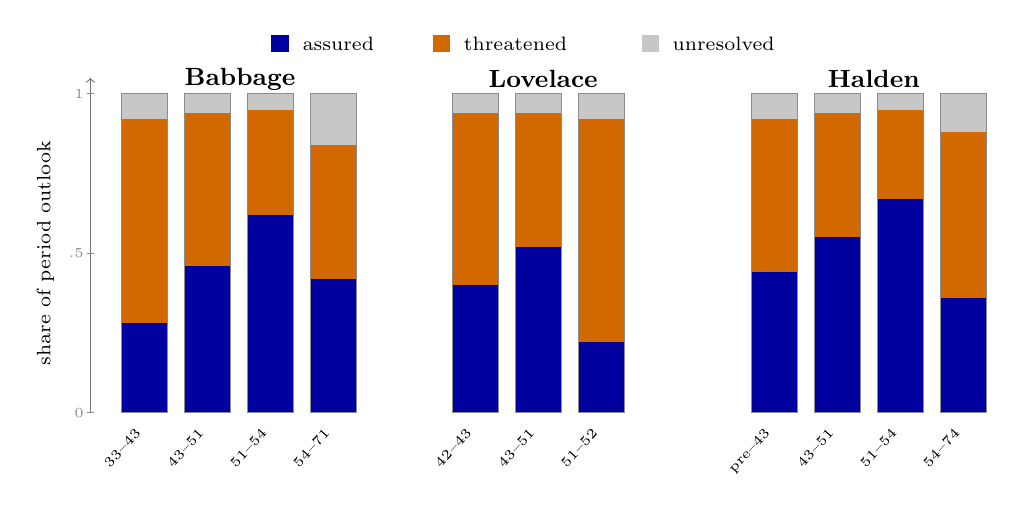
\begin{tikzpicture}[x=1cm,y=4.05cm]
  \fill[mmassured] (2.15,1.13) rectangle +(0.22,0.055);
  \node[font=\scriptsize,anchor=west] at (2.42,1.157) {assured};
  \fill[mmthreat] (4.20,1.13) rectangle +(0.22,0.055);
  \node[font=\scriptsize,anchor=west] at (4.47,1.157) {threatened};
  \fill[mmremainder] (6.85,1.13) rectangle +(0.22,0.055);
  \node[font=\scriptsize,anchor=west] at (7.12,1.157) {unresolved};

  \draw[black!55,->] (-0.15,0) -- (-0.15,1.05);
  \foreach \y/\lab in {0/0,.5/.5,1/1}
    \draw[black!45] (-0.19,\y) -- (-0.11,\y)
      node[left,font=\tiny] {\lab};
  \node[font=\scriptsize,rotate=90] at (-0.72,.5) {share of period outlook};

  \node[font=\small\bfseries] at (1.75,1.045) {Babbage};
  \MMOutlookBar{0.25}{.28}{.64}{33--43}
  \MMOutlookBar{1.05}{.46}{.48}{43--51}
  \MMOutlookBar{1.85}{.62}{.33}{51--54}
  \MMOutlookBar{2.65}{.42}{.42}{54--71}

  \node[font=\small\bfseries] at (5.60,1.045) {Lovelace};
  \MMOutlookBar{4.45}{.40}{.54}{42--43}
  \MMOutlookBar{5.25}{.52}{.42}{43--51}
  \MMOutlookBar{6.05}{.22}{.70}{51--52}

  \node[font=\small\bfseries] at (9.80,1.045) {Halden};
  \MMOutlookBar{8.25}{.44}{.48}{pre--43}
  \MMOutlookBar{9.05}{.55}{.39}{43--51}
  \MMOutlookBar{9.85}{.67}{.28}{51--54}
  \MMOutlookBar{10.65}{.36}{.52}{54--74}
\end{tikzpicture}
\endgroup
\caption{Slow fulfillment-outlook Cuts across the principals' opened periods.
Each bar divides one period-specific unit among assured fulfillment, threatened
fulfillment, and unresolved remainder. Equal bar widths show authored period
order only; they do not encode duration, intensity, probability, or measured
psychology.}
\label{fig:book-slow-outlook}
\end{figure}

\begin{figure}[htbp]
\centering
\begingroup
\colorlet{mmpath}{violet!72!black}
\newcommand{\MMSceneFrame}[2]{%
  \draw[black!55] (#1,0) rectangle ({#1+4.10},3.25);
  \foreach \a/\xx in {.2/.416,.5/2.199,.8/3.981}{%
    \draw[black!25] ({#1+\xx},0) -- ({#1+\xx},-.07)
      node[below,font=\tiny] {\a};
  }
  \foreach \t/\yy in {.2/.340,.5/1.795,.8/3.250}{%
    \draw[black!10] (#1,\yy) -- ({#1+4.10},\yy);
    \draw[black!25] (#1,\yy) -- ({#1-.07},\yy);
  }
  \begin{scope}
    \clip (#1,0) rectangle ({#1+4.10},3.25);
    \draw[black!25,densely dashed] ({#1+.119},3.25) -- ({#1+4.100},0);
    \draw[black!25,densely dashed] (#1,3.104) -- ({#1+3.803},0);
    \draw[black!25,densely dashed] (#1,2.619) -- ({#1+3.209},0);
  \end{scope}
  \node[font=\tiny] at ({#1+2.05},-.43) {assured share};
  \node[font=\small\bfseries] at ({#1+2.05},3.55) {#2};
}
\newcommand{\MMScenePoint}[6]{%
  \coordinate (#1) at
    ({#2+5.9420*((#3)-.13)},{4.8507*((#4)-.13)});
  \fill[mmpath] (#1) circle (1.8pt);
  \node[font=\tiny,fill=white,inner sep=.45pt,#6] at (#1) {#5};
}
\begin{tikzpicture}[x=1cm,y=1cm,>=Latex]
  \MMSceneFrame{0}{Babbage}
  \MMSceneFrame{4.85}{Lovelace}
  \MMSceneFrame{9.70}{Halden}
  \node[font=\scriptsize,rotate=90] at (-.70,1.63) {threatened share};
  \node[font=\tiny,anchor=east] at (-.10,.340) {.2};
  \node[font=\tiny,anchor=east] at (-.10,1.795) {.5};
  \node[font=\tiny,anchor=east] at (-.10,3.250) {.8};

  \MMScenePoint{b1}{0}{.38}{.55}{1}{above left}
  \MMScenePoint{b2}{0}{.76}{.18}{2}{above left}
  \MMScenePoint{b3}{0}{.79}{.16}{3}{below right}
  \MMScenePoint{b4}{0}{.28}{.65}{4}{above left}
  \MMScenePoint{b5}{0}{.51}{.29}{5}{above}
  \draw[mmpath,->,thin] (b1) to[bend left=10] (b2);
  \draw[mmpath,->,thin] (b2) -- (b3);
  \draw[mmpath,->,thin] (b3) to[bend right=11] (b4);
  \draw[mmpath,->,thin] (b4) to[bend left=8] (b5);

  \MMScenePoint{l1}{4.85}{.45}{.49}{1}{below right}
  \MMScenePoint{l2}{4.85}{.70}{.24}{2}{above right}
  \MMScenePoint{l3}{4.85}{.39}{.54}{3}{above left}
  \MMScenePoint{l4}{4.85}{.16}{.76}{4}{above left}
  \draw[mmpath,->,thin] (l1) to[bend left=10] (l2);
  \draw[mmpath,->,thin] (l2) to[bend left=12] (l3);
  \draw[mmpath,->,thin] (l3) to[bend right=7] (l4);

  \MMScenePoint{h1}{9.70}{.50}{.42}{1}{above left}
  \MMScenePoint{h2}{9.70}{.72}{.23}{2}{above left}
  \MMScenePoint{h3}{9.70}{.78}{.17}{3}{below right}
  \MMScenePoint{h4}{9.70}{.18}{.73}{4}{above left}
  \draw[mmpath,->,thin] (h1) to[bend left=9] (h2);
  \draw[mmpath,->,thin] (h2) -- (h3);
  \draw[mmpath,->,thin] (h3) to[bend right=12] (h4);
\end{tikzpicture}
\endgroup
\caption{Selected scene-outlook Cuts as chronological paths through a magnified
coordinate view of the same three-child simplex. Horizontal and vertical
position give assured and threatened share; the three diagonal guides give
unresolved shares of .05, .10, and .20. Babbage: negotiation, trial, expansion, returned table,
custody; Lovelace: proposal, trial, qualification, succession request; Halden:
estimate, trial, expansion, returned table. Curved arrows separate reversals
and order the elicited scenes; they do not interpolate a continuous function or
make the selected scenes an exhaustive time series.}
\label{fig:book-scene-simplex}
\end{figure}
